\section{Methodology}\label{sec_methodology}\chapter{Related Work}

\section{MITRE ATT\&CK Framework}\label{sec:related:mitre}

\section{MulVal Infrastructure Modeling}\label{sec:related:mulval}

\section{PKB}\label{sec:related:pkb}

% \subsection{Benchmarking Security Metrics}\label{sec:methodology:benchmarking}
% 
At a high level each attack graph based security metric follows the simplified processing pipeline shown in Fig \ref{fig:metric_pipeline}. 

% \begin{table}[ht]
% \centering
% \caption{Generalized Metric Pipeline}
% \label{tab:metric_proc_pipeline}
% \resizebox{.48\textwidth}{!}{%
% \toprule
% \begin{tabular}{@{}p{.20\linewidth}p{.22\linewidth}p{.22\linewidth}p{.22\linewidth}@{}}
%  1. Input & 2. Pre-Process & 3. Compute  & 4. Report \\ \midrule
%  System Model & Generate AG & Measurement &  Return values \\
% \bottomrule
% \end{tabular}
% }
% \end{table}

\begin{figure*}[ht]
\centering
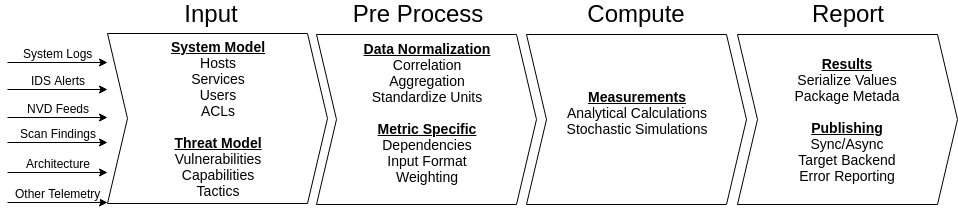
\includegraphics[width=.8\linewidth]{img/metric_calc_pipeline.png}
\caption{General Security Metric Evaluation Pipeline}
\label{fig:metric_pipeline}
\end{figure*} 

In Step 1, the inputs include host definitions, accounts and permissions, network connectivity and ACLs, system policies, vulnerability definitions, etc. It is usually assumed these parameters are collected through standard management tools and translated into a common system model for consumption by the attack graph generation engine. 

In Step 2, the system model is examined for policy violations or possible exploits that would lead to a given target's compromise. If a compromise is possible, an attack graph is produced. This is the expected input for most of the metrics we have examined, although some also assume the edges have been weighted with CVSS scores first.

The algorithm for computing the metric is run in step 3 with the attack graph as input, and the computed result is returned in the final step. 

Our first observation is that survivorship bias\cite{Wald_1980} is implicit in all AG based security metrics. An attack graph is produced \textit{only} when a system model includes in its definition enough detail to identify possible attacks. An attack graph will \textbf{not} be created if a system is totally \textit{secure}. Secure and insecure systems should, in theory at least, be mutually exclusive and collectively exhaustive; unfortunately, an attack graph will also \textbf{not} be created if a system is totally \textit{insecure}, but the system model or processing logic is incomplete. So, when validating AG metrics, we must have accepted a priori the selection bias inherent with their use. That is, we are not measuring if a system is secure or not; rather, we are measuring just how insecure that system is. 

With this in mind, validation can be seen as a test of how well a metric captures the scale of insecurity which is known to be on the system under test. We propose here a simple methodology for calibrating a metric and gauging it's accuracy in a controlled manner. 

\begin{algorithm}
\caption{Calibrate Weighted Security Metric}
\label{alg:calibrate_secmet}
\begin{algorithmic}
\REQUIRE Valid Attack Graph, N = \# partitions
\FOR{n $\in$ range (1..N)} 
 \STATE Fix all weights at $\frac{scale}{n}$ 
 \STATE Take measurement
\ENDFOR
 \end{algorithmic}
\end{algorithm}

What we assume in Algorithm \ref{alg:calibrate_secmet} is that the security metric is using some weighting scheme to influence an attacker's selection of paths, which is common in all but the structural metrics (more on these later) we've encountered. So, for CVSS base score weighted AG metrics, we would fix all vulnerabilities at the lowest score (1 in this case) and calculate the metric, and do the same again fixing all vulnerabilities at the highest score for the scale (10 for CVSS). This bounds the range of the metric under test. Creating more than 2 partitions of the score range gives us insight into the behaviour of the metric for this particular attack graph. An example of this calibration is given in \ref{sec_results}

To turn this testing algorithm into a benchmark, we need attack graphs which represent typical deployment scenarios. By far the most common use cases in the literature are small enterprise systems consisting of a limited number of distinct node types (web server, database, firewall, workstation, ...) and a 2-dimensional perimeter. While these examples are easily digestible when describing the applicability of an intensive mathematical derivation, they fall short of validating the new metric as it would be seen in the wild. We propose a standard benchmark set of attack graphs which isolate interesting attack patterns for study. In this way we can target \textit{micro-benchmarks} for specific properties, and integrate or compose models for a more rounded workload examination.

\begin{table*}[ht]
\centering
\caption{AG Standard Set - Target Scenarios}
\label{tab:ag_standard_set}
\begin{tabular}{@{}p{.15\linewidth}p{.15\linewidth}p{.15\linewidth}p{.15\linewidth}p{.15\linewidth}@{}}
\toprule
 & Enterprise & MEC/MANET &  Core &  Cloud \\ \midrule
Small (10-20) & Multi Site & UE Access  & Attachment Point & API misuse \\
Medium (100-200) & Container/K8s & 4G/5G & Layer 1\&2 & Hypervisor  \\
Large (1000-2000) & Insider/Exfil  &  IoT &  SDN/NFV & APT  \\ \bottomrule
\end{tabular}
\end{table*}



\subsection{Metric Processing Pipeline} \label{sec:methodology:input_modeling}

% \subsection{Input Modeling} \label{sec:methodology:input_modeling}
\textbf{Input Modeling}



In the \textit{Input} stage of Figure \ref{fig:automation:metric_pipeline}, system details depicted above the inbound arrows on the left are parsed into a model which describes the current environment or environment under test. Model parameters can be populated synthetically or from a live system. Rules comprising the threat model which describes how these components are allowed to interact with each other and with external stimulus can be added here for metrics that require it. The raw inputs to the processing pipeline can vary widely depending on which security metrics are being considered. At a high level, we treat the input stage as a black box for handling information requests from subsequent stages. This affords us the freedom to connect static data for testing and experimentation, and live data for production deployments without altering the contract or interface. In practice input targets can be existing APIs provided by SIEMs, query interfaces to a configuration database, source code repositories, vulnerability information feeds, generated network topologies, etc. At this stage we only assume appropriate adapters exist to make this data available for the subsequent stages.


% \subsection{PTaH: Preprocessing and Transformation Handling}
\textbf{PTaH: Preprocessing and Transformation Handling}
\label{sec:methodology:ptah_arch}

The \textit{Pre Process} stage transforms the current knowledge base into a format suitable for the desired metric calculation. 

\begin{figure}[ht]
\centering
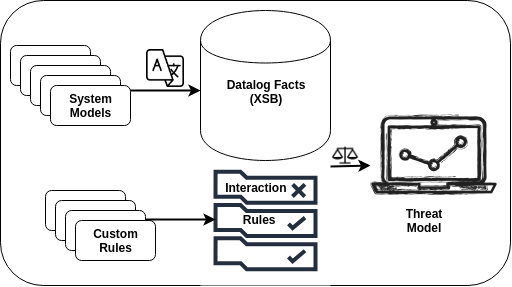
\includegraphics[width=.5\linewidth]{img/Ptah_archs.png}
\caption{Preprocessing and Transformation Handlers (\textbf{PTaH})}
\label{fig:automation:ptah_arch}
\end{figure} 

In metrics that compute aggregates, ratios, or simple statistics from findings and system facts, preprocessing steps may be minimal or bypassed entirely. In more complex metrics, such as those which consider the relationships between components or vulnerabilities, it may be necessary to craft the inputs expected from some composition of system facts along with some composition or chain of metric dependencies. In particular, metrics based on attack graphs and attack nets tend to make assumptions about the input structure which can be managed in this layer. We create these structures, score transitions, apply weights and mappings, and perform any other manipulations of our knowledge base in this layer to adhere to the input assumptions of particular metrics in this layer. 

% In order to experiment with different network architectures and exploit effects, it was necessary to reproduce each step in the process: 
% Install AG suite (MulVal, XSB) $\rightarrow$ Define AG input model (Datalog/Prolog) $\rightarrow$ Generate AG (Java, C++, ANTLR4, sed) $\rightarrow$ Import NVD (JSON, XML $\rightarrow$ SQL) $\rightarrow$ Implement custom adaptor for Stochastic Model expected input (Python, inference) $\rightarrow$ Insert transition matrix into provided R script (ctrl+c, ctrl+v) 
% After following this process precisely 2 times we understood why the AG based analytics community isn’t larger. Our immediate solution was to create a set of ansible roles and plays to automate the environment setup, test execution, and results collection entirely with a single command. This in itself lowers the barrier to entry for anyone interested in experimenting with attack graphs or looking to (quickly) reproduce our results.

% \begin{figure}[ht]
% 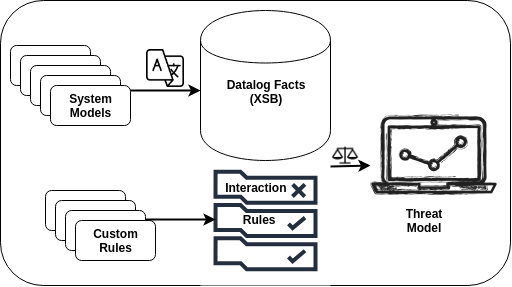
\includegraphics[width=.48\textwidth]{img/Ptah_archs.png}
% \caption{Preprocessing and Transformation Handlers (\textbf{PTaH})}
% \label{fig:automation:ptah_arch}
% \end{figure} 


% To handle the scale and volume of requests needed to support the advanced use-cases listed below, we are currently implementing and evaluating the following features in the SMaaS architecture:
% Metric Isolation: Each metric should be independently deployable to allow scaling up and down as request volume dictates. Currently metrics are bundled in Python and R modules with logical separation at the function level.






% \subsection{SecMet: A Library of Security Metrics}\label{sec:methodology:dev_env}
\textbf{SecMet: A Library of Security Metrics}

The \textit{Compute} stage implements the calculation of the security metric and takes the measurement of the current state. 

The surveys covered in Section \ref{sec:litreview} describe properties common to all the security metrics they consider, which become evaluation criteria for their review. All security metrics inherit from a parent metric class that defines these common properties and the current system model, along with housekeeping functions and metadata like citations and usage.The security metric does not contain logic to create the inputs it operates on, so we can stack metrics to run in parallel against a single source of facts, or chain them in a processing pipeline to compose more complex analytics. 

% Our architecture for implementing security metrics is straight forward. We declare a \textit{base security metric} type from which all metrics inherit three methods: 
% \begin{itemize}
% \item Check Prerequisites: is invoked either directly by the caller or in the calculate method to ensure all items necessary for the calculation are present.
% \item Calculate: returns the resulting measurement
% \item Get Metadata: returns the environment and ancillary data used during the calculation. 
% \end{itemize}
 

% \begin{figure}[H]
% \centering
% 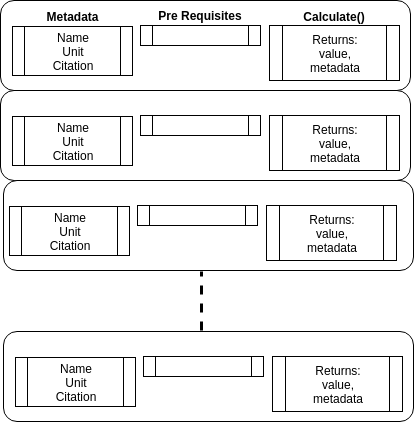
\includegraphics[width=.7\linewidth]{img/SecMet_archs.png}
% \caption{Security Metric Catalog (\textbf{SecMet})}
% \label{fig:automation:metric_arch}
% \end{figure} 

% As shown in Figure \ref{fig:automation:metric_arch}, this design allows us to implement a library of security metrics with a standard, stateless interface.


% The attack graphs described in the literature vary somewhat in structure among implementations. For example, the AGs presented in \cite{Ou_Appel_2005} include non-exploits along with exploits as nodes with edges representing lateral movements. In \cite{Noel_Jajodia_2014} the non-exploit nodes don't appear to be present in the publication, although the TVA tool isn't publicly available to test this. In \cite{Dacier_1994} and \cite{Ortalo_1999} nodes represent system privileges and edges contain exploits that grant an attacker additional privileges on a set of systems, while in \cite{Phillips_Swiler_1998} edges carry probabilities of exploitation and the nodes represent actual hosts. While the differences are subtle, they are enough to necessitate a general form of attack graph which we present in Figure \ref{fig:automation:ag_uml}. Our representation of an attack graph is a multi-edged directed acyclic graph.     

% % % \begin{wrapfigure}[10]{I}{.25\textwidth}
% % \begin{figure}[H]
% % \centering
% % 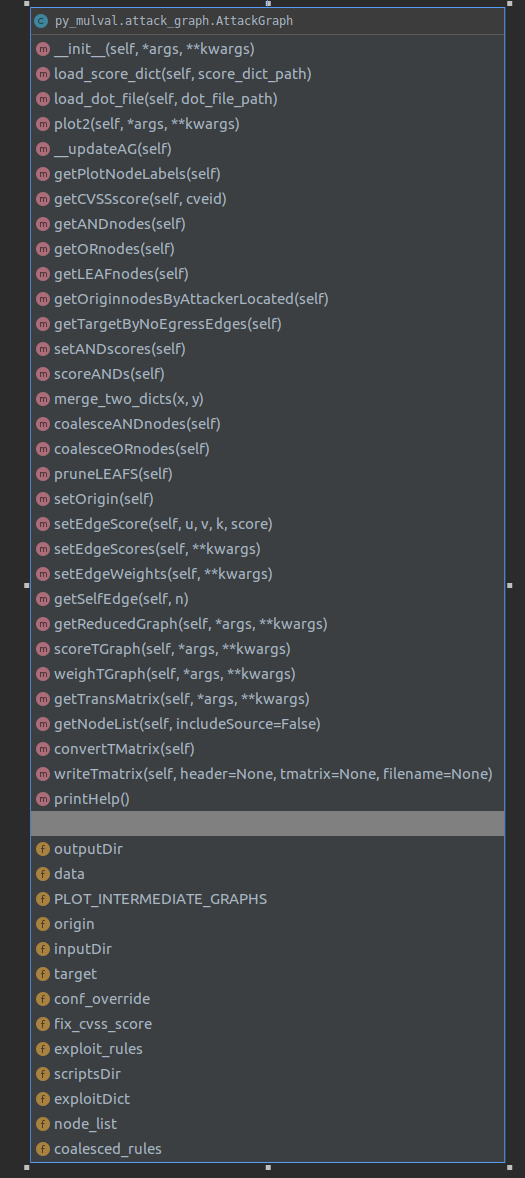
\includegraphics[scale=.45]{resource/img/ch_automation/attack_graph_class_diag.png}
% % % \end{wrapfigure}
% % \caption{Attack Graph Methods and Properties}
% % \label{fig:automation:ag_details_uml}
% % \end{figure}

% As shown in Figure \ref{fig:automation:ag_details_uml}, our implementation allows us to load various AG formats from graph description language (.dot) files, from adjacency lists as shown in Tables \ref{tab:eg_verts} and \ref{tab:eg_arcs}, or other formats as specified. Once loaded, we provide programmatic access to manipulate scoring and weighting functions, exploits definitions, and vulnerability scores. This allows for a simple means to test the range of values a metric will generate, the sensitivity of a metric to fluctuations in parameters, and how well a metric performs on different models. It also gives us some insights into how well each AG type actually models threat and defense attributes.


% \subsection{Measurement Reporting}\label{sec:methodology:reporting}
\textbf{Measurement Reporting}


Finally, the \textit{Reporting} stage handles the response logic needed to return the measured value and associated metadata appropriately. In our experience, most security metrics return a single value, although heuristics are also supported as bucket sizes and value count arrays returned within the accompanying metadata. 


% \subsection{Continuous Monitoring}\label{sec:methodology:ci}
% \input{content/methodology/continuous_monitoring.tex}

\subsection{Security Metric Validation}\label{sec:methodology:validation}





In \cite{Verendel_2009} Verendel finds 4 distinct validation methods used across the 90 security metrics papers surveyed: hypothetical, empirical, simulation, and theoretical. The author adds the caveat that no attempt was made to verify the quality of results, only to describe the methods used in each paper to substantiate the findings. In this section we propose a method for validating security metrics through empirical means.

In general, a metric should be both reliable and valid, where reliability refers to the consistency of values across repeated measurements, and validity concerns the accuracy of those values. There is currently no \textit{unit} reference for a security property which we can use for establishing the accuracy of our security metrics. We can, however, examine the behaviour of a metric relative to a given system by manipulating relevant aspects of that system while holding the other properties constant. For example, we can assign vulnerabilities to the small enterprise network shown in Figure \ref{fig:refnet_small}. For metrics that are influenced by the vulnerability score (such as CVSS based metrics), we can fix the weights of these vulnerabilities in the range of possible scores (0.0 to 10.0 in the case of CVSS). This would produce the lower and upper bound for that metric on this specific configuration of system configuration and vulnerability assignment. Similarly, we can alter properties such as the effects of a successful exploit (remote code execution, privilege escalation, etc), the placement and quantity of vulnerabilities, the underlying platform/operating system/applications, connectivity and topology, and so on. By capturing the measured values of controlled alterations to a system, we begin to understand how that metric behaves on the given system. Observing how multiple metrics behave under the same alterations allows us to compare their relative performance without an absolute point of reference. Furthermore, we can extend this analysis from a simple enterprise network to any number of use cases by supplying input adaptors for topology generators such as BRITE\cite{Medina_Lakhina_Matta_Byers_2001} or simulators like SSFNet\cite{Cowie_Ogielski_Nicol_2002} and Mininet\cite{Lantz_Heller_McKeown_2010}. Figure \ref{fig:refnets} shows an example reference set of 3 network topologies of increasing size and complexity. The first represents the type of example network commonly referenced in the literature to demonstrate a newly proposed metric, and the other two were selected from the gallery of publicly available SSFNet topologies and are described by an easy to parse domain specific language. By including systems at different scales, we are able to determine if a metric's performance depends on the size and complexity of the system under test. Intuitively, we would expect the temperature of 1 liter of boiling water to be the same as 1000 liters of boiling water, so testing against systems of varying size allows us to verify this hypothesis.

\begin{figure*}
    \centering
    \begin{subfigure}[t]{0.3\textwidth}
        % \centering
        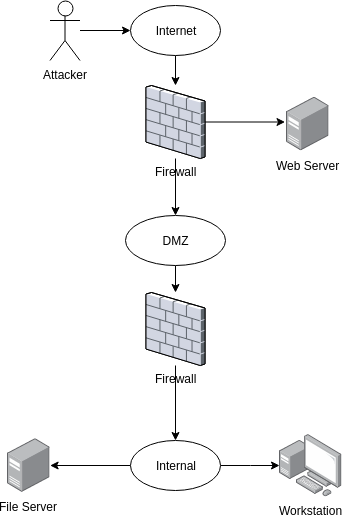
\includegraphics[width=\linewidth]{resource/img/ch_automation/from_ares_paper/net_small.png} 
        \caption{Small-sized network\cite{Ou_Appel_2005}} 
        \label{fig:refnet_small}
    \end{subfigure}
          \begin{subfigure}[t]{0.33\textwidth}
        \centering
        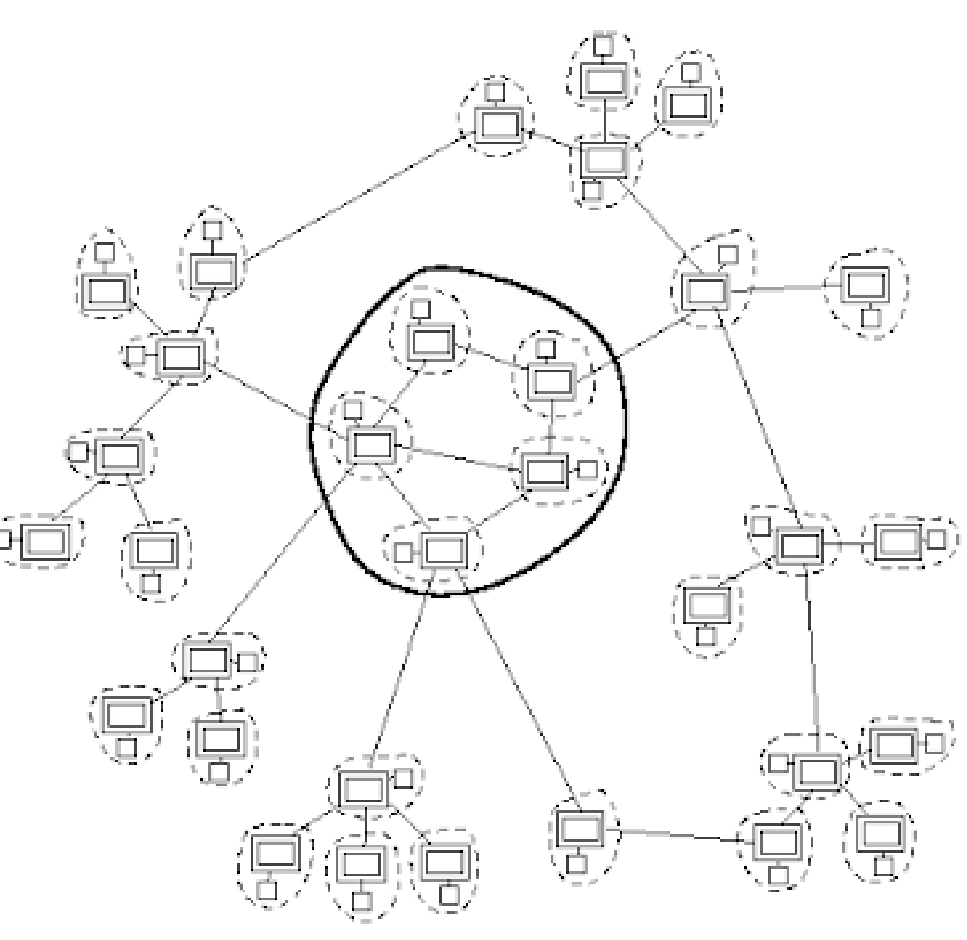
\includegraphics[width=\linewidth]{resource/img/ch_automation/from_ares_paper/net_med_2.png}
        \caption{Medium-sized network\cite{Cowie_Ogielski_Nicol_2002}}
        \label{fig:refnet_med}
    \end{subfigure}
     \begin{subfigure}[t]{0.3\textwidth}
        \centering
        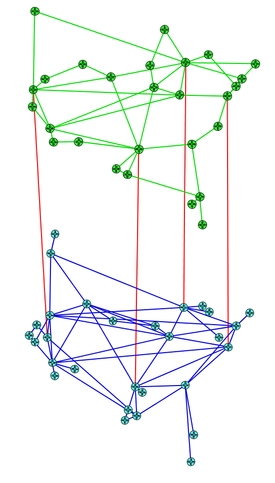
\includegraphics[width=\linewidth]{resource/img/ch_automation/from_ares_paper/net_large.png}
        \caption{Large-sized  network\cite{Cowie_Ogielski_Nicol_2002}}
        \label{fig:refnet_large}
    \end{subfigure}
    \hfill
    \caption{Different Sized Reference Networks}
    \label{fig:refnets}
\end{figure*}

If we consider a security metric as a measurement instrument, then we can validate the metric by characterizing its behavior against a reference set. Some security metric properties we might consider for validation can be taken directly from the field of measurement theory. In addition to accuracy and precision, Morris\cite{Morris_2001} describes several performance characteristics of measurement instruments that we may adapt to our validation of security metrics:

\textbf{Monotonicity}: Does the measured value always increase or always decrease with respect to each improvement in security.

\textbf{Linearity}: For security levels $s_1$ and $s_2$ and incremental security improvement $i$, is the difference between $(s_1,i)$ the same as $(s_2,i)$?

\textbf{Range}: What are the upper and lower bounds that a metric will assume for a specific model?

\textbf{Precision}: Does the metric report the same value for repeated measurements of the same quantity? This is of particular interest in probabilistic metrics. 

Analogues to other standard instrument performance measures - threshold, resolution, sensitivity to disturbance, etc - can be adapted to evaluate a security metric against our reference networks as well, and it is still to be determined which characteristics of static measurement instruments are required for their security related counterparts. 

